% !TEX program = xelatex
\documentclass[12pt,a4paper]{ctexart}
\usepackage{graphicx}
\usepackage{amsmath}
\usepackage{float}
\usepackage{geometry}
\usepackage{hyperref}
\geometry{a4paper, margin=1in}

\title{计算机图形学 HW3 实验报告：Poisson Image Editing}
\author{胡广理  学号： PB24010500}
\date{\today}

\begin{document}
\maketitle

\section{实验内容与目的}
本次实验（HW3）的主要内容是实现基于求解泊松方程的图像融合编辑（Poisson Image Editing）。实验目的包括：
\begin{itemize}
    \item 学习和实现 Poisson Image Editing 算法的核心部分：无缝融合（Seamless cloning）及带有梯度混合特性的融合（Mixing gradients）。
    \item 掌握使用 \texttt{Eigen} 库来构建并求解大规模稀疏线性方程组。
    \item 通过矩阵预分解（Cholesky 分解）技术提高求解效率，实现所选区域在目标背景上的实时拖动效果（Realtime dragging）。
\end{itemize}

\section{算法原理}

\subsection{能量泛函与变分法}
泊松图像编辑的本质是寻找一个插值函数 $f$，使得在目标区域内，它不仅能保留源图像的梯度特征，还能与目标图像的边界平滑过渡。这可以通过最小化以下能量泛函（Energy Functional）来实现：
$$ \min_{f} \iint_{\Omega} |\nabla f - \mathbf{v}|^2 \, dx dy $$
其中：
\begin{itemize}
    \item $\Omega$ 是目标图像上的待合成区域（封闭区域）。
    \item $f$ 是我们在 $\Omega$ 内部要求解的未知图像像素值（对于 RGB 图像，每一通道分别计算）。
    \item $\mathbf{v}$ 是一个给定的引导向量场（Guidance Vector Field），通常取为源图像在对应点的梯度 $\nabla g$。
\end{itemize}

为了保证生成的图像与目标图像背景边界的无缝衔接，我们需要引入狄利克雷边界条件（Dirichlet Boundary Condition）：
$$ f|_{\partial\Omega} = f^*|_{\partial\Omega} $$
其中 $\partial\Omega$ 是区域 $\Omega$ 的边界，$f^*$ 是目标图像（背景）原有的像素值。

\subsection{无缝融合（Seamless Cloning）的泊松方程推导}
根据变分法（Calculus of Variations），使得泛函 $E[f] = \iint_{\Omega} |\nabla f - \mathbf{v}|^2 \, dx dy$ 取极小值的函数 $f$，必须满足欧拉-拉格朗日方程（Euler-Lagrange Equation）。

设 $f = f_0 + \epsilon \eta$，其中 $\eta$ 是在边界 $\partial\Omega$ 上为 0 的任意光滑检验函数（即 $\eta|_{\partial\Omega} = 0$）。
将 $f$ 代入泛函求导并令微分为 0：
$$ \left. \frac{d}{d\epsilon} E[f_0 + \epsilon \eta] \right|_{\epsilon=0} = 2 \iint_{\Omega} (\nabla f_0 - \mathbf{v}) \cdot \nabla \eta \, dx dy = 0 $$
利用散度定理（Divergence Theorem）和分部积分，且考虑到 $\eta$ 在边界为 0，我们可以得到：
$$ - \iint_{\Omega} \eta \, \nabla \cdot (\nabla f_0 - \mathbf{v}) \, dx dy = 0 $$
由于 $\eta$ 在 $\Omega$ 内部是任意的，积分核必定为 0：
$$ \nabla \cdot (\nabla f - \mathbf{v}) = 0 \implies \Delta f = \nabla \cdot \mathbf{v} $$
当引导场 $\mathbf{v}$ 取为源图像的梯度 $\nabla g$ 时，$\nabla \cdot (\nabla g) = \Delta g$，这就得到了经典的泊松方程：
$$ \Delta f = \Delta g \quad \text{在 } \Omega \text{ 内部} $$
结合边界条件 $f|_{\partial\Omega} = f^*|_{\partial\Omega}$，形成了完整的边值问题。

\subsection{离散化与线性方程组}
在数字图像中，像素是定义在离散的二维网格上的。我们需要将拉普拉斯算子 $\Delta$ 离散化。对于坐标为 $p = (x, y)$ 的像素，其离散拉普拉斯算子可用四邻域近似表示为：
$$ \Delta f(p) \approx 4f(p) - \sum_{q \in N(p)} f(q) $$
其中 $N(p)$ 表示像素 $p$ 的上下左右四个相邻像素。

因此，对于选区 $\Omega$ 内部的每一个像素 $p$，泊松方程离散化为：
$$ 4f(p) - \sum_{q \in N(p) \cap \Omega} f(q) - \sum_{q \in N(p) \cap \partial\Omega} f(q) = 4g(p) - \sum_{q \in N(p)} g(q) $$

将其重排，将已知量（源图像的像素 $g$ 和边界上的目标图像像素 $f^*$）移到等号右边，未知量 $f(p)$ 留在左边：
$$ 4f(p) - \sum_{q \in N(p) \cap \Omega} f(q) = \left( 4g(p) - \sum_{q \in N(p)} g(q) \right) + \sum_{q \in N(p) \cap \partial\Omega} f^*(q) $$

如果令 $b(p) = \Delta g(p) + \sum_{q \in N(p) \cap \partial\Omega} f^*(q)$，则整个区域内的方程组可以写成矩阵形式：
$$ A \mathbf{x} = \mathbf{b} $$
这里，$\mathbf{x}$ 是包含所有未知像素点 $f(p)$ 的列向量，$A$ 是一个高度稀疏的对称正定矩阵（Sparse Symmetric Positive Definite Matrix）。这就是我们需要用 Eigen 库求解的核心线性系统。

\subsection{混合梯度（Mixing Gradients）}
当需要合成半透明或带有强纹理的对象时，源梯度的简单复制会导致目标图像背景细节丢失。通过比较源图像和目标背景的梯度，选择绝对值较大者作为指导梯度，即引导场 $\mathbf{v}$ 定义为：
$$ \mathbf{v}(p) = \begin{cases} 
      \nabla f^*(p), & |\nabla f^*(p)| > |\nabla g(p)| \\
      \nabla g(p), & \text{otherwise} 
   \end{cases} $$
然后我们求解泊松方程 $\Delta f = \nabla \cdot \mathbf{v}$。在离散情况下，公式右侧变为对应选择的梯度散度（离散拉普拉斯算子的混合版本）。这样可以使融合结果保留源图像主体特征的同时，透过主体看到目标背景的纹理。

\section{核心实现细节}

\subsection{稀疏矩阵构建与 Eigen 库使用}
引入 \texttt{Eigen::SparseMatrix} 构造多边形掩膜（mask）所对应的内部拉普拉斯稀疏矩阵。对每个 Mask 内的像素 $p$，建立该点与其四邻域 $q$ 之间关系的方程：如果是内部点，系数为 -1；若是边界之外的点，系数项即转化为边界条件并移至等号右侧方程的 $b$ 向量中。对角线系数始终为相应相接的邻居数（通常不跨画板边界为 4）。

\subsection{矩阵预计算与实时拖动优化（Precompute \& Realtime）}
如果不加优化地在每次拖拽时重建并求解方程组，算法将极其难以实现实时刷新。为解决该问题，构建了专门缓存分解结果的 \texttt{PoissonSolver} 结构：
\begin{itemize}
    \item 利用蒙版（Mask）固定的属性（即稀疏矩阵形式与拉普拉斯算子系数仅与选定区域的形状相关，与目标图像位置无关），在初次框选结束时计算稀疏矩阵并立刻通过 \texttt{Eigen::SimplicialLLT} 完成 Cholesky 预分解。
    \item 在鼠标实时拖拽的过程中触发的 \texttt{clone()} 事件，会直接重用已分解的 \texttt{solver} 来解算带有新的平移位移的坐标对应生成的独立向量 $b$（即调用 \texttt{solve(b)}）。这种处理极大降低了耗时，确保了极致平滑的实时拖拽效果。
\end{itemize}

\section{实验结果展示}
实验结果及过程图像保存于 \texttt{HW3\_images} 文件夹中，效果详细对照如下：

\begin{figure}[H]
    \centering
    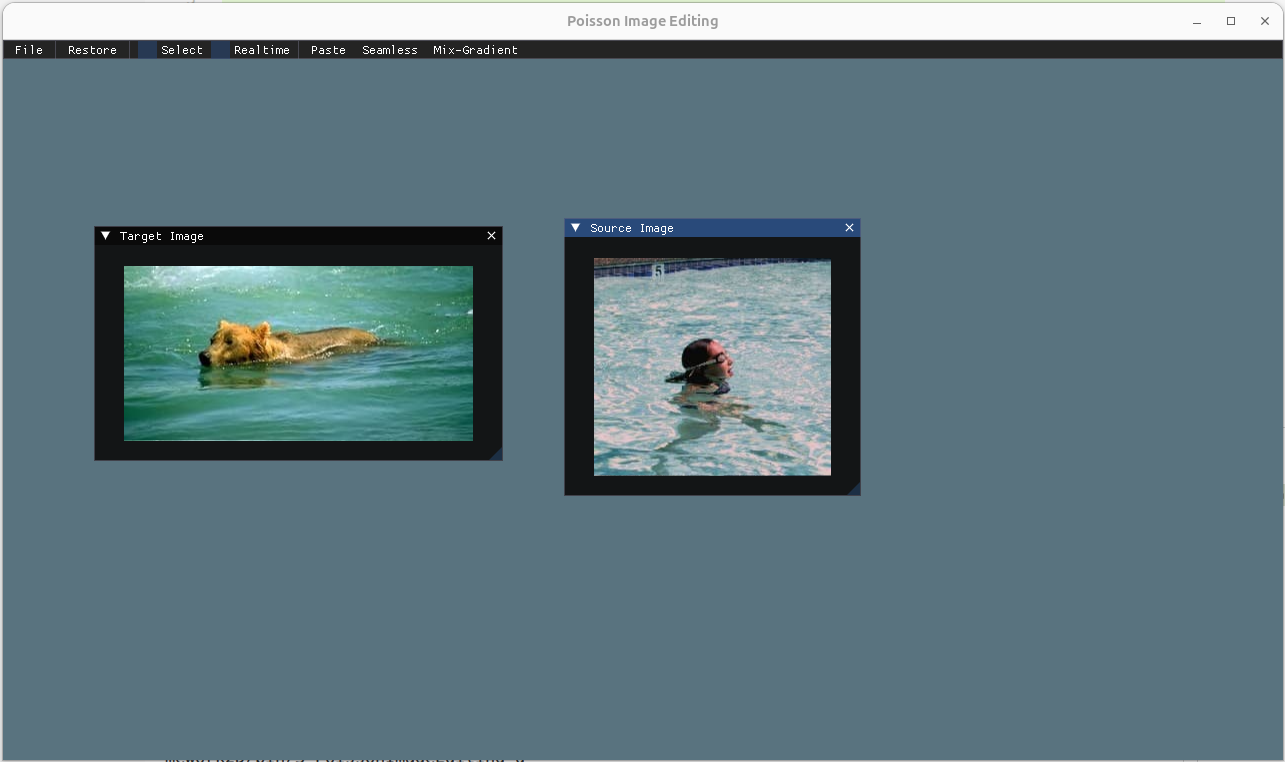
\includegraphics[width=0.45\linewidth]{HW3_images/初始的两个图像.png}
    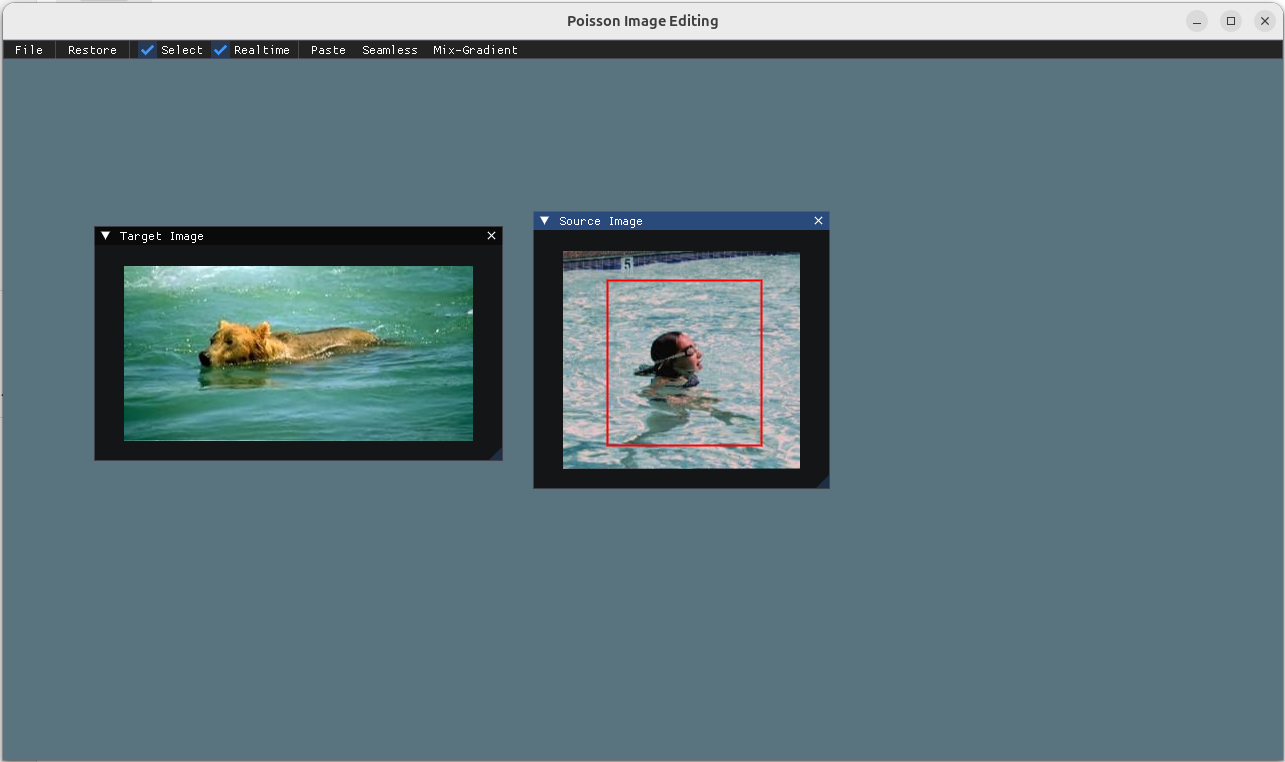
\includegraphics[width=0.45\linewidth]{HW3_images/选区域.png}
    \caption{左：系统初始载入两张图片。右：在源图像中使用工具选取待融合区域}
\end{figure}

\begin{figure}[H]
    \centering
    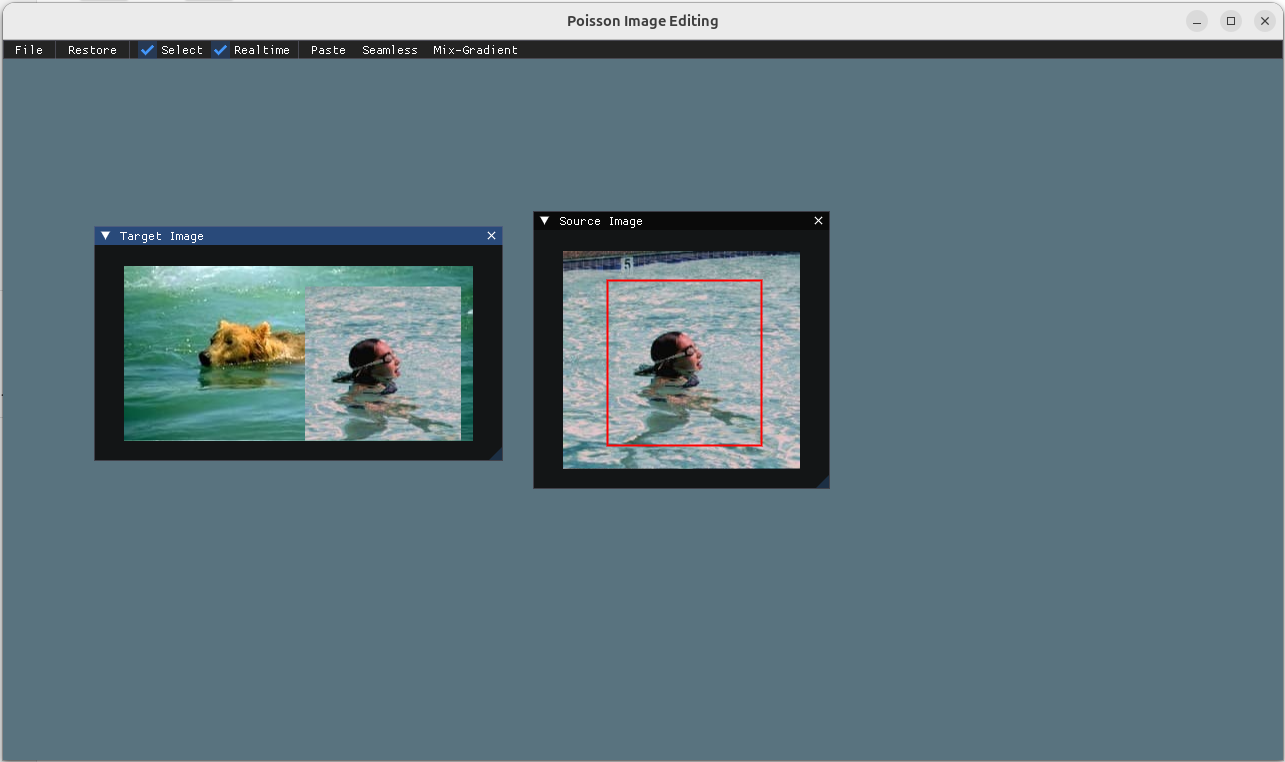
\includegraphics[width=0.6\linewidth]{HW3_images/paste.png}
    \caption{Paste（直接强行覆盖拼接）：边缘割裂感严重，颜色不匹配。}
\end{figure}

\begin{figure}[H]
    \centering
    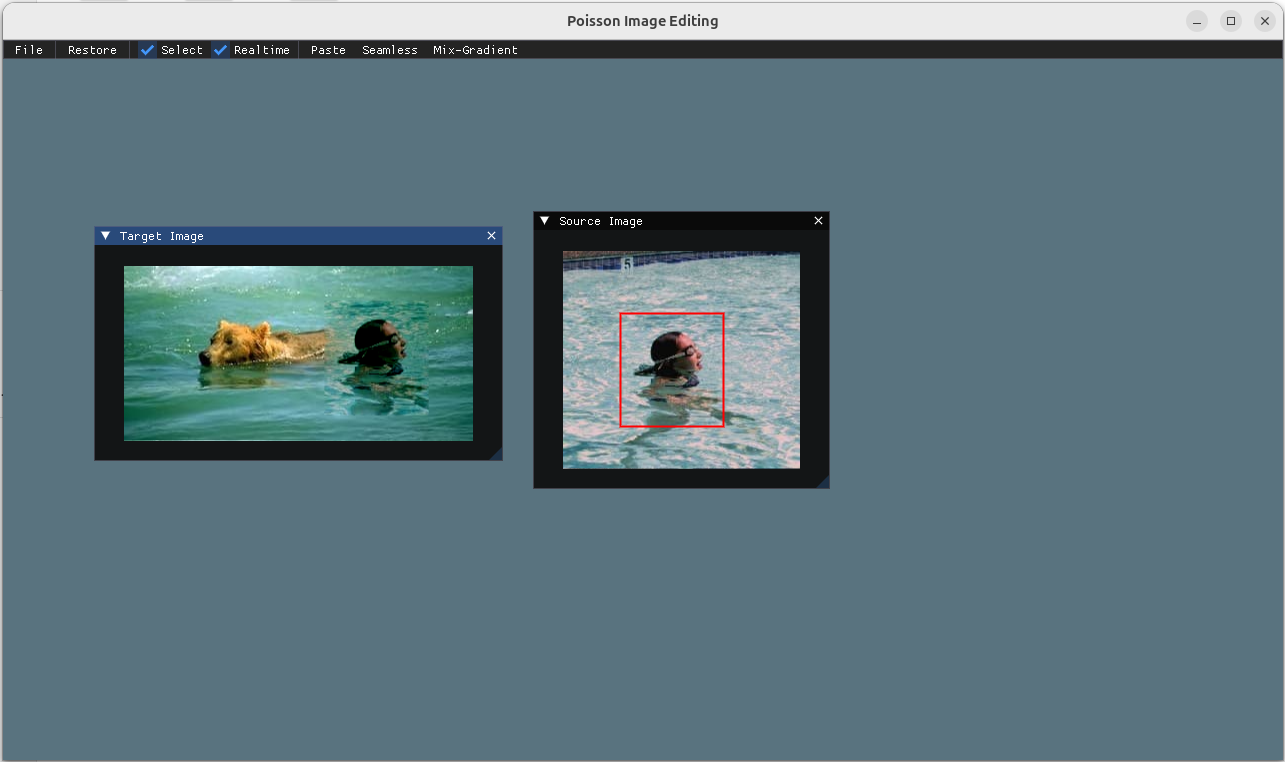
\includegraphics[width=0.6\linewidth]{HW3_images/paste+seamless.png}
    \caption{Seamless Cloning（泊松无缝融合）：边缘融合非常自然，色彩完美过渡且没有接缝。}
\end{figure}

\begin{figure}[H]
    \centering
    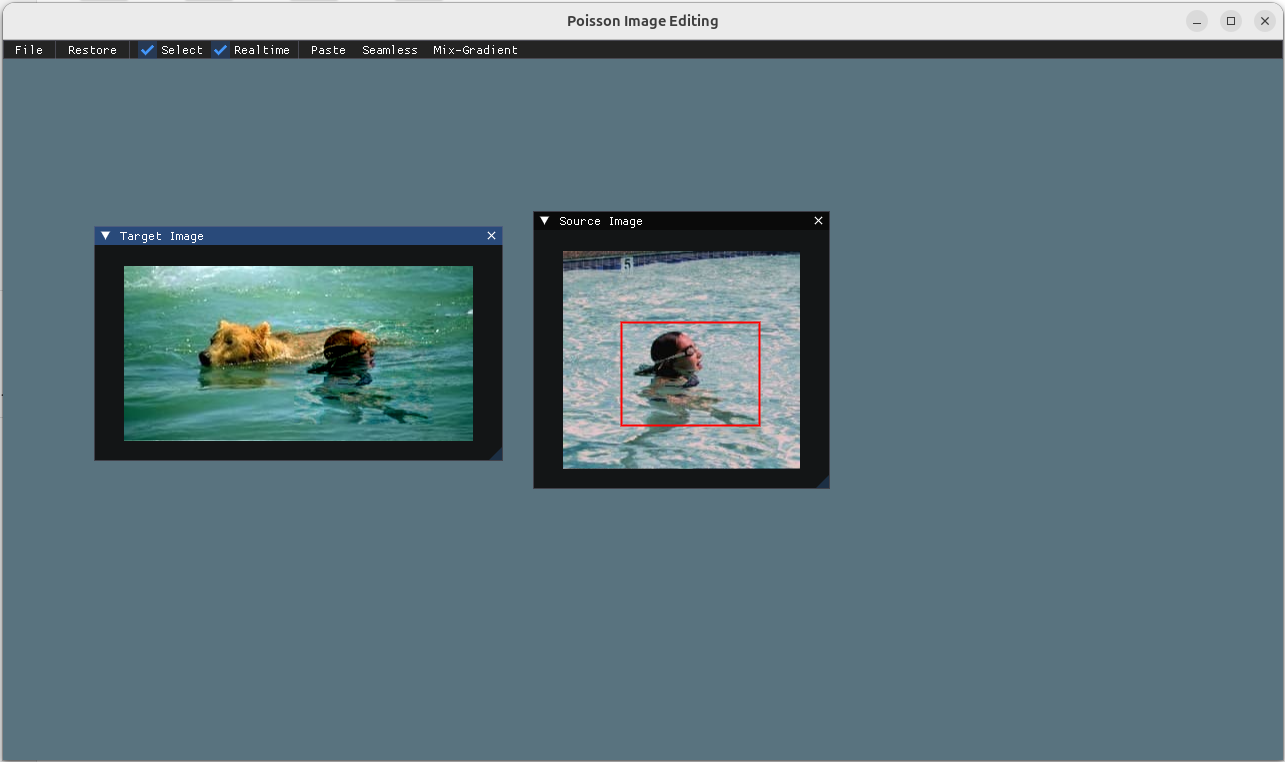
\includegraphics[width=0.6\linewidth]{HW3_images/paste+seamless+mixed.png}
    \caption{Mixing Gradients（混合梯度融合）：在无缝融合的同时，透出背景的纹理，适合半透明对象放置。}
\end{figure}

\subsection{自选图片应用结果}
同时在自己寻找的照片素材上也测试了该算法的效果，证明了算法极好的泛用能力：

\begin{figure}[H]
    \centering
    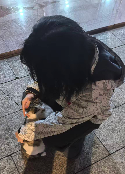
\includegraphics[width=0.4\linewidth]{HW3_images/自己找的照片.png}
    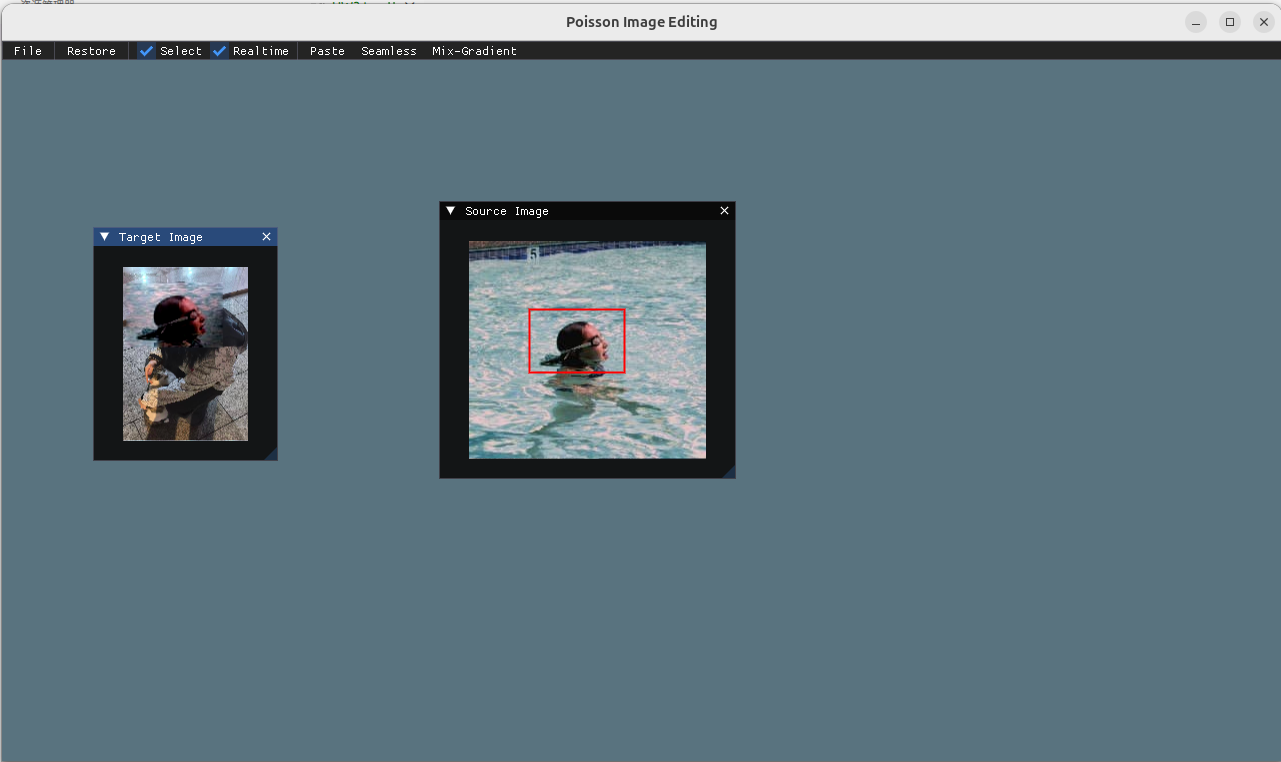
\includegraphics[width=0.55\linewidth]{HW3_images/用自己找的照片制作.png}
    \caption{左：寻找的新源图材料。右：经 Seamless Cloning 拼接到目标图像上的效果。}
\end{figure}

\section{总结}
本次实验顺利达到了预期要求，不仅正确构建且求解了泊松方程，同时巧妙运用了拉普拉斯矩阵位置不相关特性进行了 \texttt{Cholesky} 分解缓存。通过界面添加的按钮能够做到：原图复制、泊松无缝克隆、混合梯度等各效果的即时切换与顺滑的高帧率实时平移交互，加深了对稀疏方程组和图像域处理操作的理解深意。
\end{document}
